\documentclass[aspectratio=169,11pt]{beamer}

\usetheme{default}
\usepackage[T1]{fontenc}
\usepackage[lining]{CrimsonPro}
\usepackage[default]{sourcesanspro}
\usepackage{tikz}
\usepackage{graphicx}
\usepackage{booktabs}
\usepackage{textcomp}

\definecolor{ink}{RGB}{28,34,42}
\definecolor{softink}{RGB}{72,82,94}
\definecolor{accent}{RGB}{26,102,92}
\definecolor{wash}{RGB}{214,228,224}
\definecolor{paper}{RGB}{250,251,249}
\definecolor{rise}{RGB}{170,45,45}

\setbeamercolor{normal text}{fg=ink,bg=paper}
\setbeamercolor{background canvas}{bg=paper}
\setbeamertemplate{navigation symbols}{}
\setbeamertemplate{footline}{%
  \hfill{\scriptsize\color{softink}%
  \insertframenumber\,/\,\inserttotalframenumber}\hspace{6mm}\vspace{3mm}%
}
\setbeamertemplate{headline}{}
\setbeamersize{text margin left=14mm,text margin right=14mm}

\newcommand{\atmosphere}{%
  
\begin{tikzpicture}[remember picture,overlay]
    \fill[paper] (current page.south west) rectangle (current page.north east);
    \shade[left color=wash,right color=paper]
      (current page.north west) rectangle ([xshift=7.2cm]current page.south west);
    \fill[accent]
      (current page.north west) rectangle ([xshift=0.28cm]current page.south west);
    \fill[accent!14]
      ([xshift=-4.8cm]current page.north east)
      -- (current page.north east)
      -- ([yshift=-4.6cm]current page.north east)
      -- cycle;
    \node[anchor=south east,font=\scriptsize\color{softink}]
      at ([xshift=-6mm,yshift=4mm]current page.south east)
      {\insertframenumber\,/\,\inserttotalframenumber};
  \end{tikzpicture}%
}

\begin{document}

\begin{frame}[plain]
\atmosphere
\vspace{12mm}
{\fontsize{11}{14}\selectfont\color{accent}Teaching demonstration}\\[5mm]
{\rmfamily\fontsize{34}{40}\selectfont\color{ink}Understanding Inflation}\\[2mm]
{\rmfamily\fontsize{20}{26}\selectfont\color{softink}%
Why Prices Rise and\\[0.6mm]
How Central Banks Respond}\\[7mm]
{\color{accent}\rule{24mm}{1.1pt}}\\[6mm]
{\fontsize{15}{18}\selectfont\color{ink}Ke Cheng Hsu}\\[1.2mm]
{\fontsize{10.5}{13}\selectfont\color{softink}%
Ph.D.\ Candidate in Economics\\[0.2mm]
The Hong Kong University of Science and Technology}
\end{frame}

\begin{frame}[plain]
\atmosphere
\vspace{10mm}
{\fontsize{11}{14}\selectfont\color{accent}Three questions for today}\\[9mm]
{\rmfamily\fontsize{17}{24}\selectfont\color{ink}%
\begin{minipage}{0.92\textwidth}
{\tiny\color{accent}1}\hspace{2.5mm}What is inflation and how is it measured?\\[7mm]
{\tiny\color{accent}2}\hspace{2.5mm}Is inflation good or bad?\\[7mm]
{\tiny\color{accent}3}\hspace{2.5mm}What do central banks do, and at what cost?
\end{minipage}}
\end{frame}

% ---- existing receipt slide (restored; do not alter structure above) ----
\begin{frame}[plain]
\atmosphere
\vspace{2mm}
{\fontsize{11}{14}\selectfont\color{accent}A receipt from the same store, 24 years apart}\\[3mm]
\begin{columns}[T]
\column{0.34\textwidth}
\centering
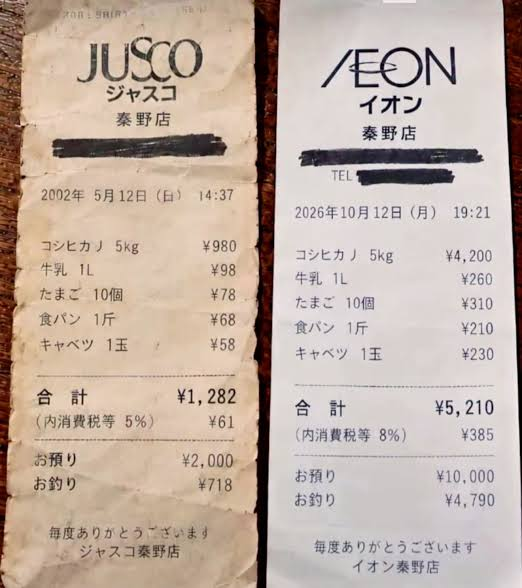
\includegraphics[width=\linewidth]{receipt.jpg}
\column{0.64\textwidth}
\centering
{\footnotesize
\begin{tabular}{@{}lrrr@{}}
\toprule
Item & 2002 & 2026 & Change\\
\midrule
Rice, 5\,kg & \textyen 980 & \textyen 4{,}200 & \textcolor{rise}{+329\%}\\
Milk, 1\,L & \textyen 98 & \textyen 260 & \textcolor{rise}{+165\%}\\
Eggs, 10 & \textyen 78 & \textyen 310 & \textcolor{rise}{+297\%}\\
Bread, 1 loaf & \textyen 68 & \textyen 210 & \textcolor{rise}{+209\%}\\
Cabbage & \textyen 58 & \textyen 230 & \textcolor{rise}{+297\%}\\
\midrule
\textbf{Total} & \textbf{\textyen 1{,}282} & \textbf{\textyen 5{,}210} & \textbf{\textcolor{rise}{+306\%}}\\
\bottomrule
\end{tabular}}

\vspace{2.5mm}
{\scriptsize\color{softink}Store: JUSCO Hadano, 12 May 2002 $\rightarrow$ AEON Hadano, 12 Oct 2026\\
(same supermarket; JUSCO was later renamed AEON)}
\end{columns}

\vspace{2.5mm}
\centering
\colorbox{wash}{\parbox{0.92\textwidth}{\centering\footnotesize
Average of the five product increases:
$(329 + 165 + 297 + 209 + 297)\,/\,5 = \textbf{259\%}$\\[2mm]
Average inflation per year (compound):
$\displaystyle
\left(\frac{\text{final}}{\text{initial}}\right)^{1/\text{years}}-1
=
\left(\frac{5210}{1282}\right)^{1/24}-1
\approx \textbf{6\%}$}}
\end{frame}

% ---- NEW: is 6% the inflation rate? ----
\begin{frame}[plain]
\atmosphere
\vspace{8mm}
{\fontsize{11}{14}\selectfont\color{accent}From the receipt to the inflation rate}\\[10mm]
\centering
{\rmfamily\fontsize{22}{30}\selectfont\color{ink}%
Do you think \textcolor{accent}{6\%}\\[2mm]
is the inflation rate?}\\[12mm]
\colorbox{wash}{\parbox{0.82\textwidth}{\centering\small\color{ink}
Milk rose 165\%; rice rose 329\%.\\
Whose basket — and how should items be weighted?}}
\end{frame}

% ---- CPI: definition, weights, formula ----
\begin{frame}[plain]
\atmosphere
\vspace{2mm}
{\fontsize{11}{14}\selectfont\color{accent}The Consumer Price Index}\\[3mm]

\begin{columns}[T]
\column{0.50\textwidth}
{\scriptsize\color{accent}1.\ Definition}\\[1.5mm]
{\rmfamily\fontsize{13}{17}\selectfont\color{ink}
The cost of a fixed basket of goods and services, relative to a base period.}\\[1.5mm]
{\scriptsize\color{softink}Basket from household spending surveys\\
(average purchases in the base year).}\\[4mm]
{\scriptsize\color{accent}2.\ Weights}\\[1.5mm]
{\footnotesize\color{ink}
Weight $=$ category spending $\div$ total spending.\\[1mm]
{\scriptsize\color{softink}Larger share of spending $\Rightarrow$ larger weight.}}\\[4mm]
{\scriptsize\color{accent}3.\ Formula}\\[1.5mm]
\colorbox{wash}{\parbox{0.95\columnwidth}{\centering\small\color{ink}
$\displaystyle
\mathrm{CPI}_t = 100\times\frac{\sum_j p_{tj}\,q_{j}}{\sum_j p_{0j}\,q_{j}}$}}\\[2mm]
{\scriptsize\color{softink}$j$ = item \textperiodcentered{}
$p_{tj}$ = today's price \textperiodcentered{}
$q_{j}$ = basket quantity}

\column{0.46\textwidth}
{\scriptsize\color{accent}What's in the basket}\\[3mm]
\centering
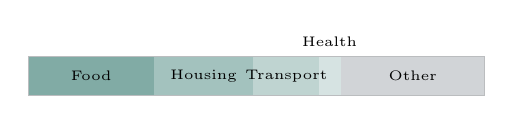
\begin{tikzpicture}[x=0.58cm,y=0.5cm]
\fill[accent!55] (0,0) rectangle (2.75,1);
\fill[accent!40] (2.75,0) rectangle (4.93,1);
\fill[accent!28] (4.93,0) rectangle (6.37,1);
\fill[accent!18] (6.37,0) rectangle (6.84,1);
\fill[softink!25] (6.84,0) rectangle (10,1);
\draw[ink!30] (0,0) rectangle (10,1);
\node at (1.38,0.5) {\tiny Food};
\node at (3.84,0.5) {\tiny Housing};
\node at (5.65,0.5) {\tiny Transport};
\node[above] at (6.6,1) {\tiny Health};
\node at (8.42,0.5) {\tiny Other};
\end{tikzpicture}\\[3mm]
{\scriptsize\color{ink}
\begin{tabular}{@{}lr@{}}
Food & 27.5\%\\
Housing & 21.8\%\\
Transport & 14.4\%\\
Health & 4.7\%\\
Other & 31.5\%\\
\end{tabular}}\\[2mm]
{\scriptsize\color{softink}Statistics Bureau of Japan, 2025 base}
\end{columns}
\end{frame}

% ---- Inflation / deflation / disinflation + formula ----
\begin{frame}[plain]
\atmosphere
\vspace{0.5mm}
{\fontsize{11}{14}\selectfont\color{accent}Inflation, Deflation, and Disinflation}\\[1mm]
{\footnotesize\color{ink}
CPI $=$ a \emph{level}.\quad
The inflation rate measures how fast that level is changing:}\\[1.2mm]
\centering
\colorbox{wash}{\parbox{0.60\textwidth}{\centering\small\color{ink}
$\displaystyle
\pi_t
=
\frac{\mathrm{CPI}_t - \mathrm{CPI}_{t-1}}{\mathrm{CPI}_{t-1}}
$}}\\[1.5mm]
{\scriptsize\color{ink}
\textbf{1. Inflation:} CPI rising ($\pi>0$).\quad
\textbf{2. Deflation:} CPI falling ($\pi<0$).\quad
\textbf{3. Disinflation:} CPI still rising, but $\pi$ falling.}\\[1.5mm]

\centering
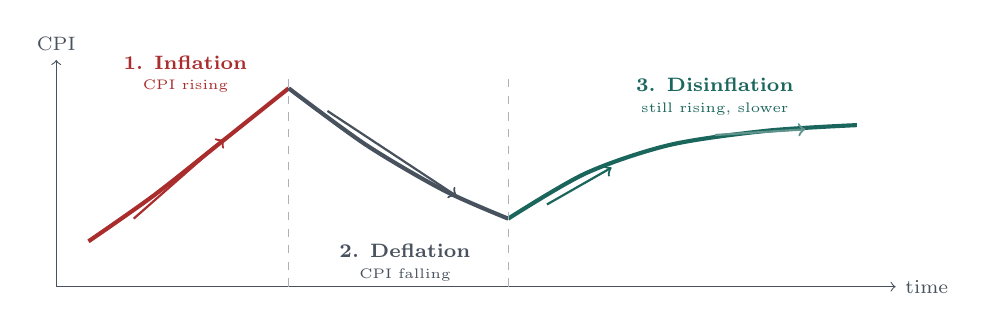
\begin{tikzpicture}[x=0.82cm,y=0.36cm]
  \draw[->,softink] (0,0) -- (13.0,0) node[right,font=\scriptsize]{time};
  \draw[->,softink] (0,0) -- (0,8.0) node[above,font=\scriptsize]{CPI};

  \draw[line width=1.5pt,rise]
    plot[smooth] coordinates
      {(0.5,1.6) (1.5,3.2) (2.5,5.0) (3.6,7.0)};
  \node[rise,font=\scriptsize,align=center] at (2.0,7.5)
    {\textbf{1. Inflation}\\[-0.5pt]{\tiny CPI rising}};
  \draw[->,rise,thick] (1.2,2.4) -- (2.6,5.2);

  \draw[line width=1.5pt,softink]
    plot[smooth] coordinates
      {(3.6,7.0) (4.8,5.0) (6.0,3.4) (7.0,2.4)};
  \node[softink,font=\scriptsize,align=center] at (5.4,0.85)
    {\textbf{2. Deflation}\\[-0.5pt]{\tiny CPI falling}};
  \draw[->,softink,thick] (4.2,6.2) -- (6.2,3.2);

  \draw[line width=1.5pt,accent]
    plot[smooth] coordinates
      {(7.0,2.4) (8.2,4.0) (9.5,5.0) (11.0,5.5) (12.4,5.7)};
  \node[accent,font=\scriptsize,align=center] at (10.2,6.7)
    {\textbf{3. Disinflation}\\[-0.5pt]{\tiny still rising, slower}};
  \draw[->,accent,thick] (7.6,2.9) -- (8.6,4.2);
  \draw[->,accent!70,thick] (10.2,5.35) -- (11.6,5.55);

  \draw[dashed,softink!45] (3.6,0) -- (3.6,7.4);
  \draw[dashed,softink!45] (7.0,0) -- (7.0,7.4);
\end{tikzpicture}
\end{frame}

% ---- Worked example: Q, table, then solution ----
\begin{frame}[plain]
\atmosphere
\vspace{0.5mm}
{\fontsize{11}{14}\selectfont\color{accent}Example: milk and rice}\\[1.5mm]
{\scriptsize\color{accent}Question}\\[1mm]
{\footnotesize\color{ink}
Basket $=$ \textbf{2\,L milk} $+$ \textbf{2 bags rice}.
Compute the CPI at $t=0,1,2$, then $\pi_1$ and $\pi_2$.
Is $t=2$ deflation?}\\[2.5mm]
{\scriptsize\color{accent}Prices}\\[1mm]
\centering
{\footnotesize
\begin{tabular}{@{}lrrr@{}}
\toprule
& $t=0$ (base) & $t=1$ & $t=2$\\
\midrule
Milk & \textyen 100 & \textyen 120 & \textyen 125\\
Rice & \textyen 200 & \textyen 240 & \textyen 250\\
\bottomrule
\end{tabular}}

\pause
\vspace{2.5mm}
{\scriptsize\color{accent}Solution}\\[1mm]
{\scriptsize\color{ink}
\begin{tabular}{@{}lrrr@{}}
\toprule
& $t=0$ & $t=1$ & $t=2$\\
\midrule
Cost $=2p_m+2p_r$ &
$2\times100+2\times200=\textbf{600}$ &
$2\times120+2\times240=\textbf{720}$ &
$2\times125+2\times250=\textbf{750}$\\
CPI $=100\times$cost$/600$ &
\textbf{100} & \textbf{120} & \textbf{125}\\
$\pi_t$ & --- &
$(120-100)/100=\textbf{20\%}$ &
$(125-120)/120\approx\textbf{4.2\%}$\\
\bottomrule
\end{tabular}}\\[2mm]
\colorbox{wash}{\parbox{0.90\textwidth}{\centering\scriptsize\color{ink}
CPI rose both periods $\Rightarrow$ \textbf{inflation}.\quad
$\pi$ fell $20\%\rightarrow4.2\%$ $\Rightarrow$ \textbf{disinflation}, not deflation.
}}
\end{frame}

% ---- Three costs of inflation ----
\begin{frame}[plain,label=costs]
\atmosphere
\vspace{1.5mm}
{\fontsize{11}{14}\selectfont\color{accent}Three costs of inflation}\\[3mm]
{\footnotesize\color{ink}
\begin{tabular}{@{}p{0.28\textwidth}p{0.62\textwidth}@{}}
{\scriptsize\color{accent}1.\ Shoe-leather}
& Cash loses value when prices rise.
People hold less cash and make more trips to the bank
--- time wasted protecting money.\\[3.5mm]
{\scriptsize\color{accent}2.\ Menu costs}
& Firms change prices more often
(menus, websites, shelves).
Prices update at different speeds
$\Rightarrow$ price confusion.\\[3.5mm]
{\scriptsize\color{accent}3.\ Unexpected inflation}
& Moves wealth around when inflation differs from expectations:
borrowers gain, lenders and fixed pensions lose.
Unpredictable inflation creates uncertainty
--- planning gets harder for everyone.\\
\end{tabular}}
\end{frame}

% ---- Benefits of inflation ----
\begin{frame}[plain,label=benefits]
\atmosphere
\vspace{1.5mm}
{\fontsize{11}{14}\selectfont\color{accent}Benefits of inflation}\\[3mm]
{\footnotesize\color{ink}
\begin{tabular}{@{}p{0.28\textwidth}p{0.62\textwidth}@{}}
{\scriptsize\color{accent}1.\ Encourage investment}
& Modest inflation makes idle cash lose a little value,
nudging people toward productive investment
(stocks, equipment, new firms).\\[4.5mm]
{\scriptsize\color{accent}2.\ Grease the job market}
& Firms rarely cut nominal pay.
With a little inflation, real wages can adjust down
without a pay cut --- helping keep unemployment lower.\\
\end{tabular}}
\end{frame}

% ---- Hyperinflation (Zimbabwe) ----
\begin{frame}[plain,label=hyperinflation]
\atmosphere
\vspace{1.5mm}
{\fontsize{11}{14}\selectfont\color{accent}Hyperinflation: Zimbabwe}\\[2.5mm]
{\footnotesize\color{ink}
\begin{tabular}{@{}p{0.24\textwidth}p{0.66\textwidth}@{}}
{\scriptsize\color{accent}What it is}
& Extremely rapid price increases
--- prices can double in hours or days.\\[3mm]
{\scriptsize\color{accent}Zimbabwe}
& 2008 peak: inflation exploded;
people abandoned the Zimbabwean dollar,
turned to foreign currency and barter.\\[3mm]
{\scriptsize\color{accent}Why}
& Money printed to cover deficits;
confidence in the currency collapsed.\\[3mm]
{\scriptsize\color{accent}Today}
& Argentina and Venezuela still hyperinflationary;
Zimbabwe's new currency is still watched closely.\\
\end{tabular}}
\end{frame}

% ---- Policy tools: interest rates ----
\begin{frame}[plain,label=tool-rates]
\atmosphere
\vspace{1.5mm}
{\fontsize{11}{14}\selectfont\color{accent}Tool 1: Interest rates}\\[1.5mm]
{\scriptsize\color{softink}Which tool to use depends on how costly inflation is.}\\[3mm]
{\footnotesize\color{ink}
\begin{tabular}{@{}p{0.28\textwidth}p{0.62\textwidth}@{}}
{\scriptsize\color{accent}Raise rates}
& Borrowing gets more expensive
$\Rightarrow$ spending and investment cool
$\Rightarrow$ demand falls
$\Rightarrow$ inflation eases.\\[4mm]
{\scriptsize\color{accent}Lower rates}
& Borrowing gets cheaper
$\Rightarrow$ spending and investment rise
$\Rightarrow$ demand rises
$\Rightarrow$ can push inflation up.\\[4mm]
{\scriptsize\color{accent}Tradeoff}
& Fighting inflation with higher rates
often means slower growth.\\
\end{tabular}}
\end{frame}

% ---- Policy tools: reserve requirements ----
\begin{frame}[plain,label=tool-reserves]
\atmosphere
\vspace{1.5mm}
{\fontsize{11}{14}\selectfont\color{accent}Tool 2: Reserve requirements}\\[1.5mm]
{\scriptsize\color{softink}The share of deposits banks must keep as reserves.}\\[3mm]
{\footnotesize\color{ink}
\begin{tabular}{@{}p{0.28\textwidth}p{0.62\textwidth}@{}}
{\scriptsize\color{accent}Raise the ratio}
& Banks must hold more cash idle
$\Rightarrow$ less lending
$\Rightarrow$ money and demand tighten
$\Rightarrow$ inflation pressure falls.\\[4mm]
{\scriptsize\color{accent}Lower the ratio}
& Banks can lend more
$\Rightarrow$ credit expands
$\Rightarrow$ spending can rise
$\Rightarrow$ inflation pressure rises.\\[4mm]
{\scriptsize\color{accent}Idea}
& Control credit at the source
--- how much banks are allowed to create.\\
\end{tabular}}
\end{frame}

% ---- Policy tools: yield curve control (Japan) ----
\begin{frame}[plain,label=tool-ycc]
\atmosphere
\vspace{1.5mm}
{\fontsize{11}{14}\selectfont\color{accent}Tool 3: Yield curve control}\\[1.5mm]
{\scriptsize\color{softink}Japan's case --- pinning long-term interest rates.}\\[3mm]
{\footnotesize\color{ink}
\begin{tabular}{@{}p{0.28\textwidth}p{0.62\textwidth}@{}}
{\scriptsize\color{accent}What it is}
& The central bank targets not only short rates,
but also long-term bond yields.\\[3.5mm]
{\scriptsize\color{accent}Bank of Japan}
& Bought government bonds as needed
to keep long yields near a target
--- cheap long-term borrowing.\\[3.5mm]
{\scriptsize\color{accent}Why}
& When short rates are already near zero,
YCC tries to keep stimulus flowing
through the whole yield curve.\\
\end{tabular}}
\end{frame}

% ---- Diagnosing the cause ----
\begin{frame}[plain,label=causes]
\atmosphere
\vspace{2mm}
{\fontsize{11}{14}\selectfont\color{accent}Diagnosing the cause}\\[1.5mm]
{\scriptsize\color{softink}Three channels --- illustrations from the United States.}\\[4mm]
{\footnotesize\color{ink}
\begin{tabular}{@{}p{0.22\textwidth}p{0.68\textwidth}@{}}
{\scriptsize\color{accent}1.\ Demand}
& COVID ``helicopter money'': cash sent to households
$\Rightarrow$ spending rises faster than supply
$\Rightarrow$ prices are pulled up.\\[4mm]
{\scriptsize\color{accent}2.\ Supply}
& Oil shocks (Gulf / Hormuz) and trade wars:
higher energy costs, tariffs, broken chains
$\Rightarrow$ costs rise
$\Rightarrow$ prices are pushed up.\\[4mm]
{\scriptsize\color{accent}3.\ Expectations}
& Inflation high
$\Rightarrow$ workers expect higher prices
$\Rightarrow$ demand higher wages
$\Rightarrow$ firms pass on costs
$\Rightarrow$ inflation stays high
$\Rightarrow$ \ldots\\
\end{tabular}}
\end{frame}

% ---- Output--inflation tradeoff ----
\begin{frame}[plain,label=tradeoff]
\atmosphere
\vspace{2mm}
{\fontsize{11}{14}\selectfont\color{accent}The output--inflation tradeoff}\\[2.5mm]
\colorbox{wash}{\parbox{0.90\textwidth}{\centering\footnotesize\color{ink}
Different causes need different responses.\\
Fighting a supply shock only by cutting demand
can cause \textbf{stagflation}.
}}\\[4mm]
\begin{columns}[T]
\column{0.48\textwidth}
{\scriptsize\color{accent}Demand-driven}\\[1.5mm]
{\footnotesize\color{ink}
Raise rates
$\Rightarrow$ spending cools
$\Rightarrow$ inflation falls.\\[2mm]
{\scriptsize\color{softink}Cost: slower growth.}}
\column{0.48\textwidth}
{\scriptsize\color{accent}Supply-driven}\\[1.5mm]
{\footnotesize\color{ink}
Oil / trade war:
prices \textcolor{rise}{up},
output \textcolor{rise}{down}
--- \textbf{stagflation}.\\[2mm]
{\scriptsize\color{softink}Cutting demand alone deepens the slump.}}
\end{columns}
\end{frame}

% ---- Japan case study: CPI chart ----
\begin{frame}[plain,label=japan-chart]
\atmosphere
\vspace{0.5mm}
{\fontsize{11}{14}\selectfont\color{accent}Case study: Japan's CPI inflation over time}\\[1mm]
{\scriptsize\color{softink}Annual \% change in consumer prices.
Source: World Bank via FRED (series FPCPITOTLZGJPN).}\\[1.5mm]
\centering
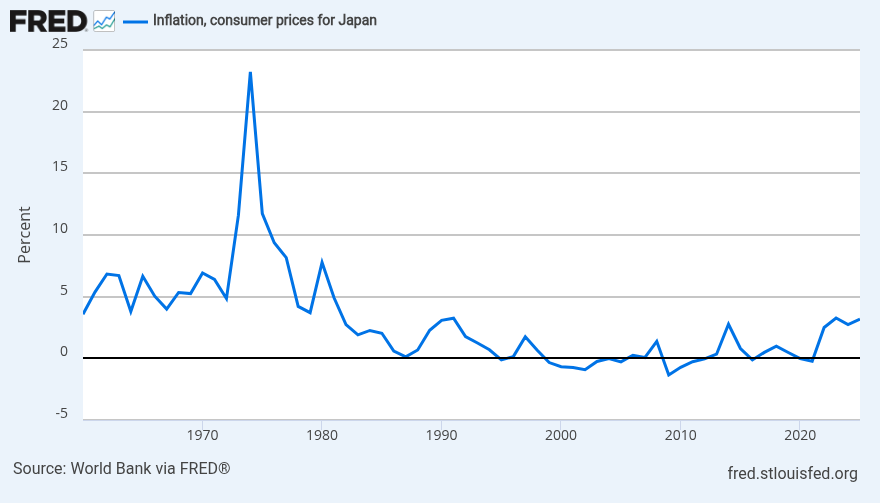
\includegraphics[width=0.92\textwidth,height=0.62\textheight,keepaspectratio]{japan_cpi_inflation_fred.png}\\[1mm]
{\scriptsize\color{ink}
\textbf{Periods to read:}
bubble peak $\sim$1990 $\rightarrow$
long near-zero/negative stretch $\rightarrow$
2008--09 dip $\rightarrow$
2013--14 uptick $\rightarrow$
COVID dip $\rightarrow$
2022+ pickup.}
\end{frame}

% ---- Japan case study: early periods ----
\begin{frame}[plain,label=japan-early]
\atmosphere
\vspace{1mm}
{\fontsize{11}{14}\selectfont\color{accent}Reading the chart: bubble, deflation, 2008}\\[2mm]
{\footnotesize\color{ink}
\begin{tabular}{@{}p{0.28\textwidth}p{0.62\textwidth}@{}}
{\scriptsize\color{accent}1.\ Bubble $\sim$1990}
& Late-1980s stock and land boom;
BOJ raised rates in 1989--90;
equity prices collapsed in 1990.
CPI inflation was still about 3\% in 1990--91,
then faded as the bust hit balance sheets.\\[3mm]
{\scriptsize\color{accent}2.\ Long deflation}
& CPI inflation turned negative in 1995
and stayed near zero or below for years:
weak demand, bad loans, and expectations
that prices would keep falling.\\[1.5mm]
& BOJ response: zero rates (1999),
QE (2001), then QQE / negative rates / YCC (2013--16).\\[3mm]
{\scriptsize\color{accent}3.\ 2008--09 dip}
& Inflation briefly positive in 2008,
then about $-1.4\%$ in 2009
--- oil prices crashed after the 2008 surge,
and demand weakened in the global crisis.\\
\end{tabular}}
\end{frame}

% ---- Japan case study: recent periods ----
\begin{frame}[plain,label=japan-recent]
\atmosphere
\vspace{1mm}
{\fontsize{11}{14}\selectfont\color{accent}Reading the chart: Abenomics, COVID, turnaround}\\[2mm]
{\footnotesize\color{ink}
\begin{tabular}{@{}p{0.28\textwidth}p{0.62\textwidth}@{}}
{\scriptsize\color{accent}4.\ 2013--14 uptick}
& April 2013: QQE and a 2\% price target.
2014 CPI rose about 2.7\%,
but much of that was the consumption-tax hike
(5\%$\rightarrow$8\%); underlying inflation stayed softer.\\[3mm]
{\scriptsize\color{accent}5.\ COVID dip}
& All-items CPI: 0.0\% in 2020, $-0.2\%$ in 2021
--- prices slipped again during the pandemic lull.\\[3mm]
{\scriptsize\color{accent}6.\ 2022+ pickup}
& Core CPI (excl.\ fresh food) above 2\% since April 2022.
Drivers: weaker yen, imported energy costs,
then stronger wages (2024 spring talks: largest in decades).\\[1.5mm]
& March 2024: BOJ ended negative rates and YCC
--- from fighting deflation to managing inflation.\\
\end{tabular}}
\end{frame}

\end{document}
